\documentclass[tikz,border=10pt]{standalone}
\usepackage{tikz}
\usetikzlibrary{shapes,arrows,positioning,shadows,fit}

\begin{document}

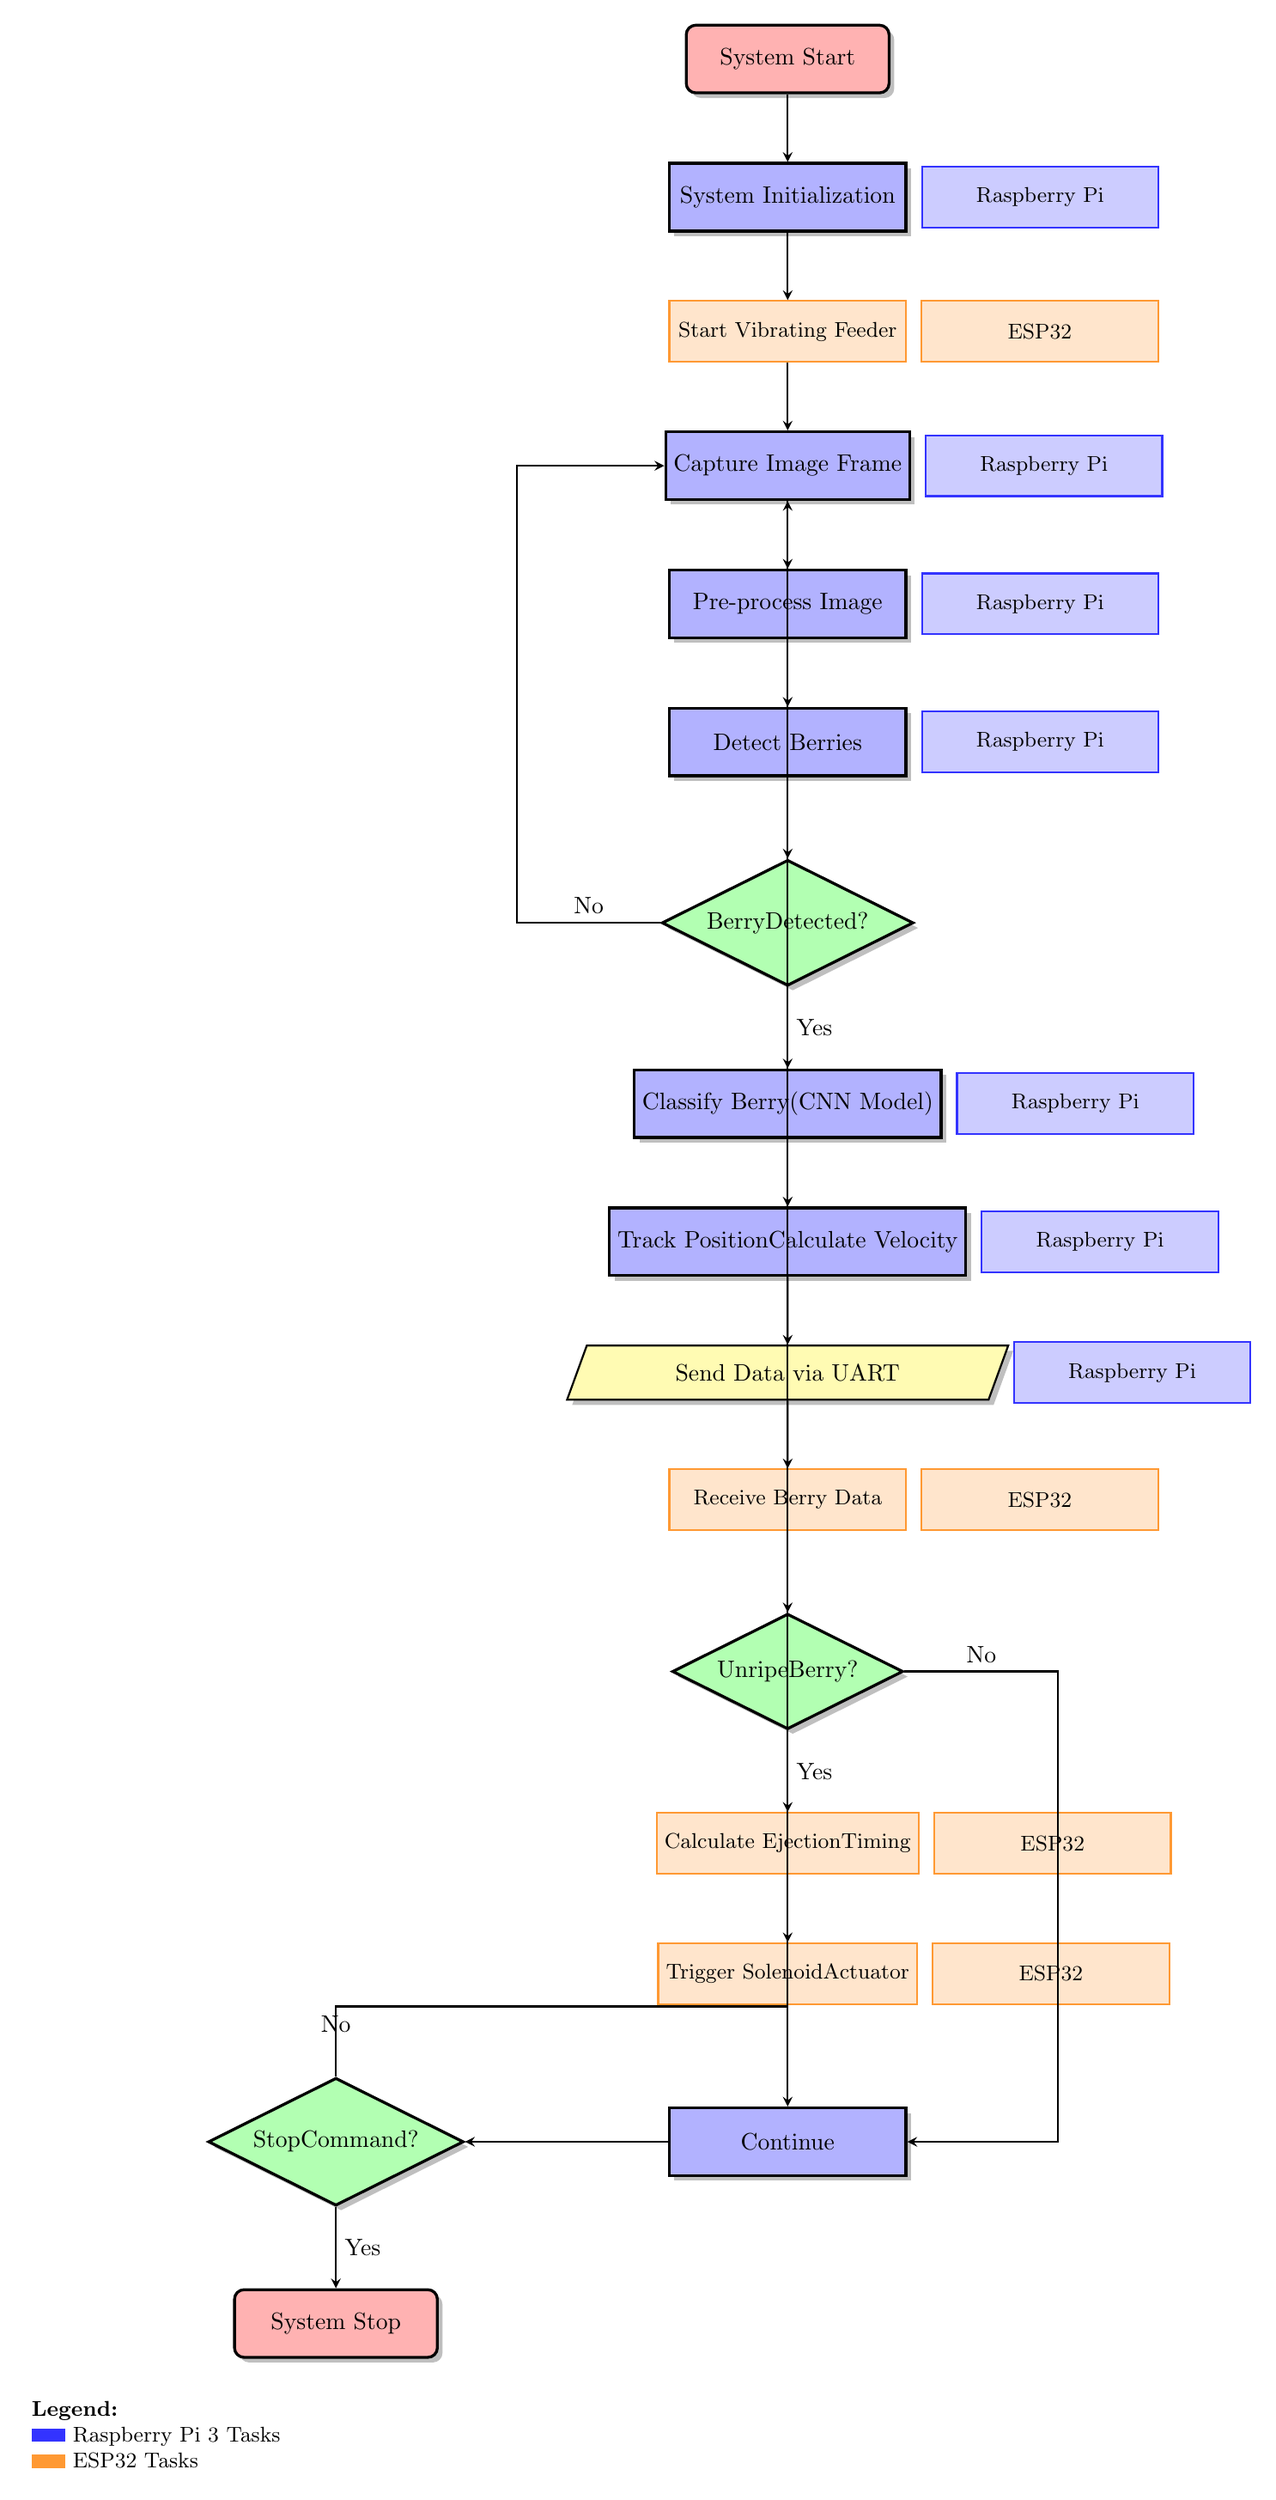
\begin{tikzpicture}[
    node distance=1cm,
    startstop/.style={rectangle, rounded corners, minimum width=3cm, minimum height=1cm, text centered, draw=black, fill=red!30, drop shadow, very thick},
    process/.style={rectangle, minimum width=3.5cm, minimum height=1cm, text centered, draw=black, fill=blue!30, drop shadow, very thick},
    decision/.style={diamond, minimum width=3cm, minimum height=1cm, text centered, draw=black, fill=green!30, drop shadow, very thick, aspect=2},
    io/.style={trapezium, trapezium left angle=70, trapezium right angle=110, minimum width=3cm, minimum height=0.8cm, text centered, draw=black, fill=yellow!30, drop shadow, thick},
    rpiprocess/.style={rectangle, minimum width=3.5cm, minimum height=0.9cm, text centered, draw=blue!80, fill=blue!20, thick, font=\small},
    esp32process/.style={rectangle, minimum width=3.5cm, minimum height=0.9cm, text centered, draw=orange!80, fill=orange!20, thick, font=\small},
    arrow/.style={thick,->,>=stealth}
]

% Start
\node[startstop] (start) {System Start};

% Initialization
\node[process, below=of start] (init) {System Initialization};
\node[rpiprocess, right=0.2cm of init] (initlabel) {Raspberry Pi};

% Start motors
\node[esp32process, below=of init] (motor) {Start Vibrating Feeder};
\node[esp32process, right=0.2cm of motor] (motorlabel) {ESP32};

% Image capture loop
\node[process, below=of motor] (capture) {Capture Image Frame};
\node[rpiprocess, right=0.2cm of capture] (captlabel) {Raspberry Pi};

% Image processing
\node[process, below=of capture] (preprocess) {Pre-process Image};
\node[rpiprocess, right=0.2cm of preprocess] (prelabel) {Raspberry Pi};

% Object detection
\node[process, below=of preprocess] (detect) {Detect Berries};
\node[rpiprocess, right=0.2cm of detect] (detlabel) {Raspberry Pi};

% Decision: Berry detected?
\node[decision, below=1.2cm of detect] (detected) {Berry\\Detected?};

% Classification
\node[process, below=1.2cm of detected] (classify) {Classify Berry\\(CNN Model)};
\node[rpiprocess, right=0.2cm of classify] (classlabel) {Raspberry Pi};

% Tracking
\node[process, below=of classify] (track) {Track Position\\Calculate Velocity};
\node[rpiprocess, right=0.2cm of track] (tracklabel) {Raspberry Pi};

% Send to ESP32
\node[io, below=of track] (send) {Send Data via UART};
\node[rpiprocess, right=0.2cm of send] (sendlabel) {Raspberry Pi};

% ESP32 receives
\node[esp32process, below=of send] (receive) {Receive Berry Data};
\node[esp32process, right=0.2cm of receive] (reclabel) {ESP32};

% Decision: Reject berry?
\node[decision, below=1.2cm of receive] (reject) {Unripe\\Berry?};

% Calculate timing
\node[esp32process, below=1.2cm of reject] (timing) {Calculate Ejection\\Timing};
\node[esp32process, right=0.2cm of timing] (timelabel) {ESP32};

% Trigger solenoid
\node[esp32process, below=of timing] (eject) {Trigger Solenoid\\Actuator};
\node[esp32process, right=0.2cm of eject] (ejlabel) {ESP32};

% Continue
\node[process, below=of eject, yshift=-0.5cm] (continue) {Continue};

% End condition
\node[decision, left=3cm of continue] (end) {Stop\\Command?};

% Stop
\node[startstop, below=1.2cm of end] (stop) {System Stop};

% Arrows
\draw[arrow] (start) -- (init);
\draw[arrow] (init) -- (motor);
\draw[arrow] (motor) -- (capture);
\draw[arrow] (capture) -- (preprocess);
\draw[arrow] (preprocess) -- (detect);
\draw[arrow] (detect) -- (detected);
\draw[arrow] (detected) -- node[right] {Yes} (classify);
\draw[arrow] (detected) -- node[above] {No} ++(-4,0) |- (capture);
\draw[arrow] (classify) -- (track);
\draw[arrow] (track) -- (send);
\draw[arrow] (send) -- (receive);
\draw[arrow] (receive) -- (reject);
\draw[arrow] (reject) -- node[right] {Yes} (timing);
\draw[arrow] (reject) -- node[above] {No} ++(4,0) |- (continue);
\draw[arrow] (timing) -- (eject);
\draw[arrow] (eject) -- (continue);
\draw[arrow] (continue) -- (end);
\draw[arrow] (end) -- node[right] {Yes} (stop);
\draw[arrow] (end) -- node[above] {No} ++(0,2) -| (capture);

% Legend
\node[below=0.5cm of stop, xshift=-2cm, text width=5cm, font=\small] (legend) {
    \textbf{Legend:}\\
    {\color{blue!80}\rule{0.5cm}{0.2cm}} Raspberry Pi 3 Tasks\\
    {\color{orange!80}\rule{0.5cm}{0.2cm}} ESP32 Tasks
};

\end{tikzpicture}

\end{document}
